\documentclass[11pt,a4paper]{article}
\usepackage[T1]{fontenc}
\usepackage[utf8]{inputenc}
\usepackage[margin=23mm]{geometry}
\usepackage{graphicx,longtable,booktabs,listings,xcolor,textcomp,hyperref}
\hypersetup{colorlinks=true,linkcolor=blue,urlcolor=blue,pdftitle={TPC cosmic-test analysis manual}}
\lstset{basicstyle=\ttfamily\small,breaklines=true,columns=fullflexible,keepspaces=true,upquote=true,showstringspaces=false,frame=single,backgroundcolor=\color{black!3}}
\setlength{\parindent}{0pt}
\setlength{\parskip}{6pt}
\setlength{\emergencystretch}{3em}
\newcommand{\manualrevision}{83b6e70d01d9}

\title{TPC cosmic-test analysis\\User and modification guide}
\author{User and developer reference: Python and C++/ROOT}
\date{\today\\Source revision: \texttt{\manualrevision}}
\begin{document}
\maketitle
This manual covers detector mapping, raw inspection, event displays, manual cleaning,
and the independent voltage study. Configuration excerpts, command help and example
figures are refreshed by the manual builder. All commands below run from the workspace
root, unless an absolute path is supplied. The original input ROOT files are read-only.
\tableofcontents
\newpage

\section{Workspace and requirements}
\begin{longtable}{p{.32\linewidth}p{.62\linewidth}}
\toprule Location & Purpose \\\midrule
\texttt{data/root/} & Input files, named \texttt{ntupleNNNN.root}.\\
\texttt{analysis/} & Working Python interface: \texttt{tpc.py}, \texttt{detector.py}, \texttt{voltage.py}.\\
\texttt{analysis\_root/} & Native ROOT interface: \texttt{TPC.C} and \texttt{TPCDetector.h}. No Python is called.\\
\texttt{config/} & Shared detector cuts, independent study cuts, 1D binning and 2D pair definitions.\\
\texttt{results/python/}, \texttt{results/root/} & Outputs, grouped by workflow and run.\\
\texttt{docs/} & This LaTeX source, PDF, example figures, generated excerpts and builder.\\
\texttt{bundles/} & Shareable source bundles. Carry the sibling \texttt{config/} and \texttt{docs/} folders when sharing. Input data are not bundled.\\
\bottomrule
\end{longtable}
ROOT requires C++17. Python requires PyROOT, NumPy and Matplotlib; interactive Python
windows also require a working TkAgg backend. File-only Python exports use
\texttt{-{}-batch}. ROOT uses \texttt{-b} for batch mode; omit \texttt{-q} when you want
an interactive ROOT session to remain open. PDF rebuilding additionally requires
Python and \texttt{pdflatex} with the standard packages used in this source.

\section{Quick start: inspect one run}
The normal inspection opens both groups together: a 1D summary and seven individual
1D canvases, plus a 2D summary and four individual 2D canvases (13 windows for the
present branch set). Data are read once per combined invocation. Python uses one
shared mapping and selection before entering one window loop.
\begin{lstlisting}
root -l 'analysis_root/TPC.C()'                     # menu
root -l 'analysis_root/TPC.C("raw",1616)'           # 1D + 2D
root -l 'analysis_root/TPC.C("raw --1d",1616)'
root -l 'analysis_root/TPC.C("raw --2d",1616)'
root -l 'analysis_root/TPC.C("raw-clean",1616)'     # both, cleaned

python analysis/tpc.py                              # menu
python analysis/tpc.py raw 1616                     # both
python analysis/tpc.py raw 1616 --1d
python analysis/tpc.py raw 1616 --2d
python analysis/tpc.py raw 1616 --apply-cuts
python analysis/tpc.py raw 1616 --batch              # save, no windows
\end{lstlisting}
ROOT dimension flags belong \emph{inside the quoted command string}. Python also
accepts \texttt{-{}-dimensions both|1d|2d} (or \texttt{-{}-dim}).
Raw inspection bypasses all manual cuts and automatic event vetoes. Cleaned inspection
uses the detector database and that run's event-veto ledger. Mapping applies in both.
The old \texttt{raw2d} / \texttt{raw2d-clean} commands remain 2D-only shortcuts.

\subsection{Focus and export locations}
\begin{lstlisting}
root -l 'analysis_root/TPC.C("raw:Channel",1616)'
root -l 'analysis_root/TPC.C("raw2d:Charge_vs_Pad",1616)'
python analysis/tpc.py raw 1616 --branches Channel
python analysis/tpc.py raw 1616 --plots Charge_vs_Pad
python analysis/tpc.py raw 1616 --1d --branches Time --range 80 100
\end{lstlisting}
Focused exports use \texttt{branches\_NAME/} or \texttt{plots\_NAME/} subfolders so
that they preserve full-run outputs. Specify \texttt{-{}-dimensions both} in Python
when combining focused selections from both groups. Both engines save ordinary
outputs in \texttt{results/ENGINE/raw/runNNNN/}; cleaned outputs add
\texttt{cleaned/}, and 2D outputs add \texttt{2d/}.

\section{Command and option reference}
The menus provide the same operations as the command interface. ROOT arguments are
\texttt{TPC(command,run,event,inputDirectory,outputDirectory,vetoCSV,cutsDB,studyCutsDB)}.
Empty strings retain defaults. Dimension flags belong inside the ROOT command string.
\begin{longtable}{p{.22\linewidth}p{.27\linewidth}p{.41\linewidth}}
\toprule ROOT command & Python command & Effect \\\midrule
raw & raw RUN & Uncut 1D and 2D inspection together; saves files and opens windows.\\
raw -{}-1d / raw -{}-2d & raw RUN -{}-1d / -{}-2d & Select one inspection group; -{}-both explicitly requests both.\\
raw-clean & raw RUN -{}-apply-cuts & Both groups with detector DB cuts and existing automatic veto IDs applied.\\
raw-clean -{}-1d / -{}-2d & raw RUN -{}-apply-cuts -{}-1d / -{}-2d & Cleaned inspection of one group.\\
raw:Channel (or another field) & raw RUN -{}-branches Channel & Focused 1D original-channel diagnostic. raw:Pad uses mapped pads.\\
raw2d:NAME & raw RUN -{}-plots NAME & Focused 2D pair from the pair CSV.\\
raw2d / raw2d-clean & raw2d RUN [-{}-apply-cuts] & Backwards-compatible 2D-only shortcuts.\\
cuts & cuts RUN & List active manual rules only; does not apply them or open plots.\\
event / event3d & event RUN [-{}-mode 3d] & Browse the present physical event display with detector cleaning and vetoes.\\
save & event RUN -{}-save & Export an event. ROOT exports both modes; Python exports the selected mode.\\
examples & examples & Export established run1615/event42535 and run1616/event5584 displays. Other input files are needed if not bundled.\\
voltage & voltage & Independent voltage comparison; freshly classifies event noise, then applies detector and study cuts.\\
info & info & Report paths, mapping and configuration.\\
check & check & Configuration/mapping regression checks; no data-cleaning plots.\\
\bottomrule
\end{longtable}
\begin{longtable}{p{.35\linewidth}p{.57\linewidth}}
\toprule Python option & Meaning \\\midrule
-{}-batch & Save inspection outputs without opening windows. In ROOT use -b; use -q only when automatic exit is wanted.\\
-{}-dimensions both|1d|2d & Select inspection groups; -{}-dim is an alias. -{}-1d, -{}-2d and -{}-both are short forms.\\
-{}-branches FIELD [FIELD ...] & Focus on named 1D quantities; alone it selects 1D.\\
-{}-plots NAME [NAME ...] & Focus on configured 2D pairs; alone it selects 2D.\\
-{}-bins N / -{}-bin-width W & Override 1D bin count or width (mutually exclusive).\\
-{}-range LOW HIGH & Set 1D plotting edges; does not create a cut.\\
-{}-log-y / -{}-linear-y & Override the 1D count-axis scale. 2D colour scaling uses LogZ in its CSV.\\
-{}-binning-file PATH & Alternate base 1D axis CSV, also inherited by 2D axes.\\
-{}-plots-file PATH & Alternate 2D pair/axis CSV.\\
-{}-input-dir / -{}-output-dir & Select input directory and output root; see generated help for command-specific layout.\\
-{}-pad-map PATH & Alternate Python mapping table. ROOT uses its auxiliary table.\\
-{}-cuts-db PATH & Complete replacement detector DB, including global rules; used only for cleaned data/displays.\\
-{}-veto-file PATH & Explicit precomputed run/event veto ledger.\\
-{}-event ID & Event to browse/export; otherwise the first eligible event is used.\\
-{}-save / -{}-mode 2d|3d & Event export and display mode.\\
-{}-example RUN:EVENT & Repeat to select Python examples.\\
-{}-study-cuts-db PATH & Additional independent voltage-study restrictions only.\\
-{}-voltage-file PATH & Alternate run/voltage assignments.\\
-{}-voltage-override RUN=VOLTS & Resolve an ambiguous assignment; repeatable.\\
-{}-exclude-run RUN & Exclude a run from voltage overlays.\\
-{}-noise-channels / -{}-module-channels / -{}-module-synchronous & Override noise detection thresholds during Python voltage processing; regenerate the ledger afterwards.\\
\bottomrule
\end{longtable}
Use -{}-help on the Python command for its full syntax. The appendix contains generated
help from the current implementation. ROOT path/DB overrides are positional, as
shown in the files section.

\section{Data and detector mapping}
Each input row is a recorded pulse. Multiple rows can belong to the same event or
channel. The tree is named \texttt{ntuple}. Branches used by the analysis are:
\begin{longtable}{p{.20\linewidth}p{.73\linewidth}}
\texttt{Event} & Stored event identifier; a pulse count is not an event count.\\
\texttt{Channel} & Original zero-based ROOT electronics channel.\\
\texttt{Hit} & Stored pulse index; the 2D Hit view uses this value, not the total pads in an event.\\
\texttt{Time} & Stored time value in native units.\\
\texttt{Charge} & Stored charge/amplitude value in native units; no energy calibration is assumed.\\
\texttt{Pedestal} & Stored pedestal value.\\
\texttt{Blockhead} & Additional stored field, deliberately omitted from inspection plots.\\
\end{longtable}
The established wiring table is \texttt{auxiliary/pad\_map.csv} in each engine's
folder. Printed fADC labels start at 1; \textbf{fADC = ROOT Channel + 1}.
Pad numbers start at 0, increase left to right and bottom to top, and continue from
medium pads 0--249 to large pads 250--409. Examples: fADC153 = Channel152 = Pad0;
fADC16 = Channel15 = Pad24; fADC505 = Channel504 = Pad250.

Mapping is a coordinate conversion, independent of cuts. Unconnected channels have
\texttt{Pad=-1}. Their hits are retained in flow cells of Pad histograms. Other
raw distributions, including the separate Channel diagnostic and time/charge
correlations, retain those hits. \texttt{pad\_map\_used.csv} records the wiring used.
\textbf{Do not add or subtract 1 from a Pad number.}

\section{Detector-cleaning database}
Edit \texttt{config/run\_cuts.ini}. It contains only common \texttt{[global]} and
per-run \texttt{[run NNNN]} blocks. Write conditions for values to \emph{reject}:
\begin{lstlisting}
[global]
reject = Time >= 228
reject = Channel in 271,149

[run 1616]
# Illustrations only: enable after inspecting this run.
# reject = Channel == 152
# reject = Event in 1000..1020
# reject = Pad == 42 && Time >= 90 && Time < 95
# reject = Charge > 3500
\end{lstlisting}
Separate lines are OR: a hit matching any rejection line is removed. Conditions
joined by \texttt{\&\&} on one line are AND. Operators are
\texttt{== != < <= > >=}, \texttt{in}, and \texttt{not in}.
Lists use commas; \texttt{in 40..45} includes both endpoints. A histogram interval
with edges 90 and 95 is \texttt{Time >= 90 \&\& Time < 95}.
A leading \texttt{\#} disables a line and also starts an inline comment.
There are no arbitrary functions, parentheses, or \texttt{||}; add another rejection
line for OR. Invalid syntax and missing branches produce explicit errors.

\subsection{Channels, fADC and pads in cuts}
\texttt{Channel == 152}, \texttt{FADC == 153}, and \texttt{Pad == 0} are equivalent
ways to reject the same connected pad. One is sufficient. Rejections act on hit rows
before populating \emph{all} cleaned plots, including mapped Pad plots. A pure Event
rule removes every matching event's row; a Channel/Time rule removes only matching
pulses. Fields are case-insensitive and also support Hit, Charge, Pedestal and
Blockhead. Numeric thresholds may be signed, fractional or scientific notation.
\begin{lstlisting}
python analysis/tpc.py cuts 1616
root -l 'analysis_root/TPC.C("cuts",1616)'
\end{lstlisting}
These commands \textbf{list rules only}; they do not open plots or run an analysis.
To apply the listed detector rules and display both groups, run:
\begin{lstlisting}
root -l 'analysis_root/TPC.C("raw-clean",1616)'
python analysis/tpc.py raw 1616 --apply-cuts
\end{lstlisting}
Keep any custom input/DB path overrides in the plotting command. Event displays
apply the detector rules automatically. Uncut \texttt{raw} bypasses them.
Reopen/re-run the command after DB edits. Uncut inspection intentionally ignores the
DB. The current detector database is reproduced in Appendix A.

\subsection{Automatic event-noise vetoes: detection and application}
\textbf{An automatic veto is an event-level cut: every pulse with that run/event ID
is removed when vetoes are enabled. The original ROOT file is never modified.}
Detection and application are separate steps.

\paragraph{What is detected.}
The classifier uses all original pulses and all electronics channels, including
unconnected ones, before Time/Channel/Charge cuts or pad mapping. Let $D$ be the
number of distinct channels in an event. The current setup has eight electronics
modules, with module number $\lfloor\mathrm{Channel}/72\rfloor$.
For each module define $C$ as its number of distinct channels, $H$ as its total
pulse rows, and $S$ as the largest number of distinct channels sharing exactly
the same stored Time value. Multiple pulses on one channel do not increase $D$, $C$
or the synchronous-channel count $S$.

With the present settings, veto the event if \emph{either}:
\begin{enumerate}
\item $D\ge288$ (detector-wide occupancy); or
\item any module has $C\ge58$ and also either $S\ge50$ or $H\ge3C$
(module flooding with exact-time synchrony or repeated pulses).
\end{enumerate}
There is no time-window tolerance in $S$: equality is on the stored Time value.
A module is an electronics group, not a physical pad row. These are heuristic noise
criteria; a veto is a classification under these thresholds, not a fitted physics
track decision. The settings keys are noise\_channels, module\_channels,
module\_synchronous, module\_hits\_per\_channel, channels\_per\_module and
readout\_modules. Each engine reads its own settings.csv. Changing one copy does
not change the other. The current settings are reproduced in the appendix.

\paragraph{When the veto is applied.}
\begin{longtable}{p{.40\linewidth}p{.50\linewidth}}
\toprule Command/workflow & Automatic event veto behaviour \\\midrule
ROOT raw / raw -{}-1d / raw -{}-2d; Python raw without -{}-apply-cuts; raw2d shortcuts &
\textbf{OFF}. All raw pulses remain, including flooded events. No manual cuts are applied either.\\
ROOT raw-clean; Python raw -{}-apply-cuts (1D or 2D) &
\textbf{ON, using the existing veto ledger}. Entire matching events are removed in addition to detector DB cuts.\\
Event/event3d, save and examples & \textbf{ON, using the existing ledger}, before selecting the first passing pulse per channel for display.\\
Independent voltage study & \textbf{Detects afresh} from each available listed run's full input, applies the resulting vetoes and writes a new ledger. Its separate study hit cuts do not restrict the noise-classifier input.\\
cuts & Lists manual DB rules only. It neither detects noise nor opens data plots.\\
\bottomrule
\end{longtable}
Thus, \textbf{a raw plot is deliberately not noise-cleaned}. This allows examination
of the events that would be removed. To see the effect, compare raw and raw-clean
with identical binning. Mapping remains active in both; mapping does not itself
remove noisy events.

\paragraph{Where the veto IDs come from.}
The ledger is keyed by \texttt{(run,event)}, never event number alone. Python prefers
\path{results/python/voltage/rejected_events.csv}; ROOT prefers the equivalent under
its configured output root. Otherwise the engine uses its bundled auxiliary ledger
(Python also accepts the former legacy layout). An explicit veto override takes
precedence. CSV evidence includes distinct-channel occupancy, total pulses,
detector-wide flags and per-module flooding evidence.

\textbf{Cleaned inspection does not rerun the automatic classifier.} It reads the
IDs already present in this ledger. If a run has no rows in the ledger, no automatic
IDs are vetoed for that run; an empty run entry is not evidence that a new dataset
was scanned. If the ledger is missing, cleaning raises an error. For new data,
regenerate the ledger using the voltage workflow with the relevant run listed, or
supply a validated run/event CSV using -{}-veto-file (Python) or vetoCSV (ROOT).
After changing noise thresholds, regenerate the ledger: changing settings alone
cannot change IDs in an existing file. Explicitly override the ledger when unrelated
input files reuse the same run numbers. Ordinary detector DB edits take effect on
the next cleaned invocation; they do not regenerate the automatic ledger.

\section{One-dimensional histograms and annotations}
The 3-by-2 summary shows Event, Pad, Hit, Time, Charge and Pedestal. Each has an
individual canvas. Original Channel (0--575) is an additional independent diagnostic,
including unconnected inputs. All histograms count \textbf{Raw Hits}.

\textbf{Underflow} counts values below the lower edge; \textbf{Overflow} counts values
at or above the upper edge. Every bin uses ROOT's half-open interval
\([\mathrm{low},\mathrm{high})\), including the last bin.
\textbf{Hits on unconnected channels} counts selected pulses with no assigned pad.
Those hits contribute to Pad underflow but appear at their actual Channel coordinates
in the electronics plot. Counts have thousands separators.

Edit \texttt{raw\_binning.csv}: Branch, BinWidth, Bins, Min, Max, LogY. Empty bounds
use the uncut extent. Bins takes precedence over BinWidth. Min/Max are plotting
edges, not cuts. Raw and cleaned versions use the same axis extent. Python's
\texttt{-{}-bins}, \texttt{-{}-bin-width}, \texttt{-{}-range}, and \texttt{-{}-log-y}/
\texttt{-{}-linear-y} override the 1D view for one call.
\begin{figure}[p]
\centering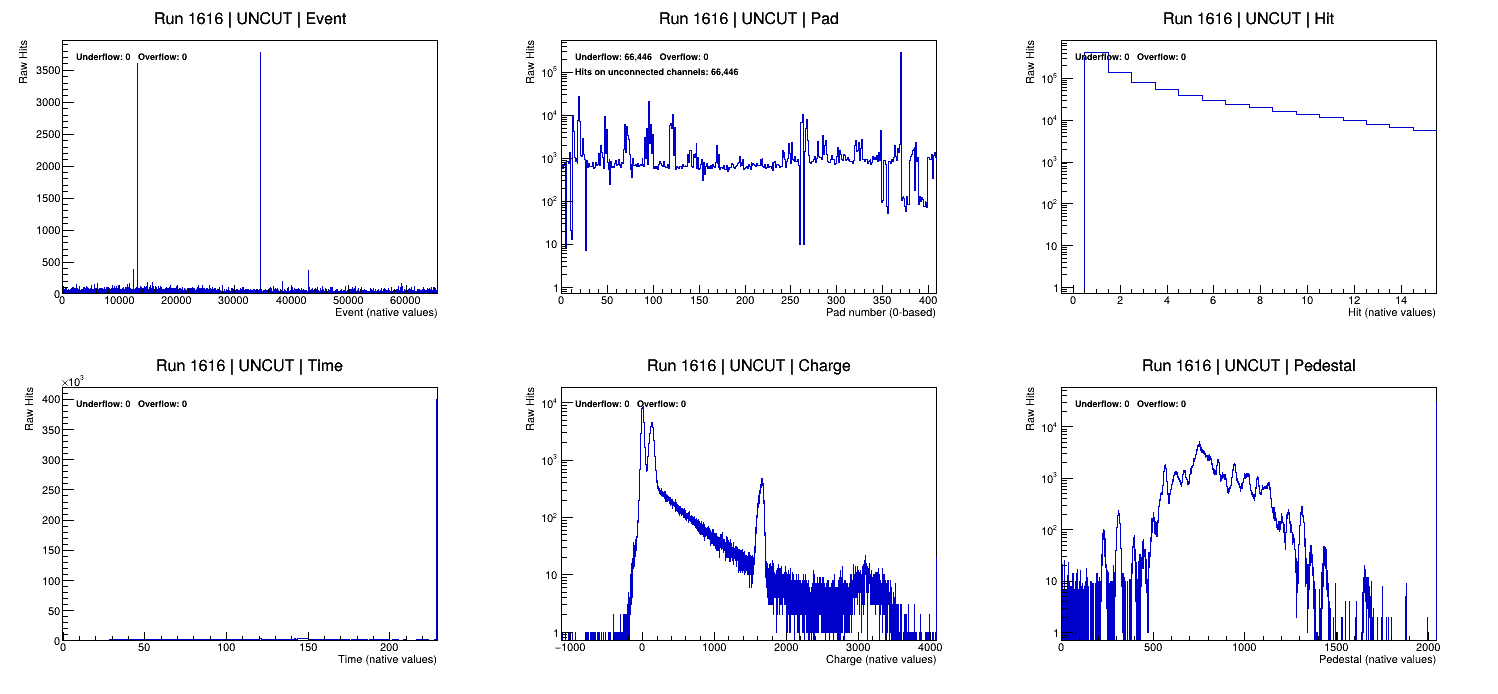
\includegraphics[width=\linewidth]{figures/raw_1d.png}
\caption{Run 1616 uncut 1D summary; generated using the current ROOT palette and settings.}
\end{figure}

\section{Two-dimensional histograms}
A 2-by-2 summary and one individual canvas per configured pair show correlations.
The colour scale counts Raw Hits, with logarithmic colour enabled by LogZ.
Empty cells are white. X/Y axes remain linear. All accepted pulses contribute;
there is no first-hit-per-channel reduction.

The following table is generated from the \emph{current} pair file, including the
configured orientation and overrides. Empty options inherit 1D binning.
\begin{longtable}{p{.27\linewidth}p{.12\linewidth}p{.12\linewidth}p{.33\linewidth}}
\textbf{Name} & \textbf{X} & \textbf{Y} & \textbf{Overrides} \\\hline
Event\_vs\_Pad & Pad & Event & YBinWidth=64, LogZ=true \\
Hit\_vs\_Pad & Pad & Hit & LogZ=true \\
Charge\_vs\_Pad & Pad & Charge & LogZ=true \\
Charge\_vs\_Time & Time & Charge & LogZ=true \\
\end{longtable}

Edit \texttt{raw\_2d\_plots.csv} to change/add pairs. X/Y define horizontal/vertical
fields. XBinWidth, XBins, XMin, XMax and corresponding Y options override each axis.
An explicit count takes precedence over a width. The plot Name controls filenames
and focused selection and must be unique and filename-safe. Python
\texttt{-{}-plots-file} chooses an alternate pair file.

For individual-event resolution in a narrower region, set YBinWidth=1, YMin=8000,
YMax=9000 on an Event-on-Y row. These edges do not change the DB.
A four-million-cell limit prevents accidental enormous dense histograms; narrow the
range or increase bin width when needed. The default event grouping in the shipped
file was chosen for a manageable overview; the current file always takes precedence.

\textbf{Outside plotted ranges} counts each hit once, including hits outside both
axes. ROOT retains all flow cells and corners; per-axis flow totals can overlap.
Sparse CSVs contain all nonzero cells, including flows: bin 0 is underflow, N+1 is
overflow, and open-end bounds are infinite. A correlation with no Pad axis retains
unconnected-channel hits in its ordinary cells if within the plotted limits.
\begin{figure}[p]
\centering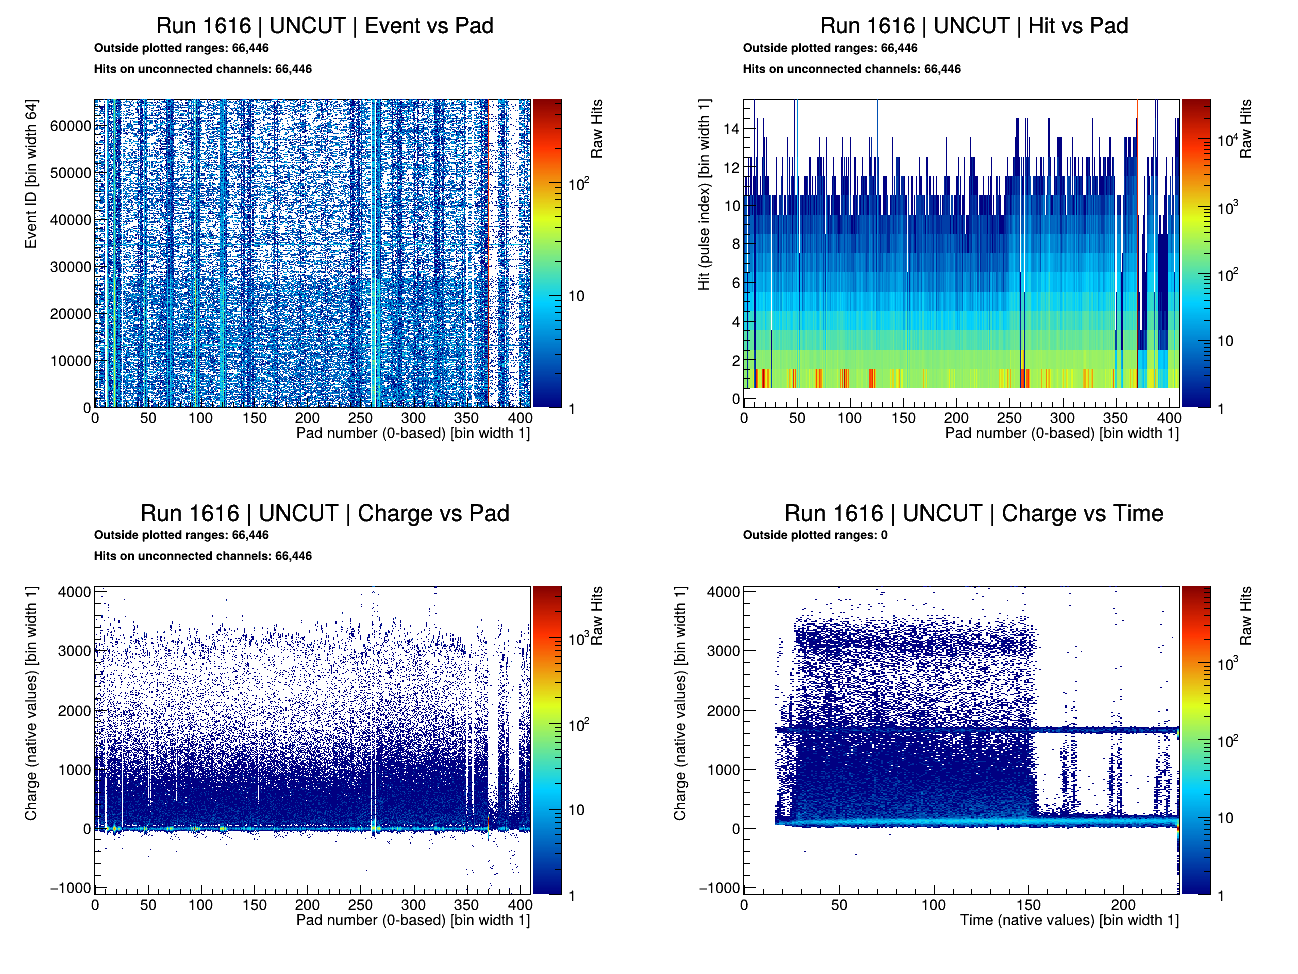
\includegraphics[width=\linewidth]{figures/raw_2d.png}
\caption{Run 1616 uncut 2D summary. Axis orientation and resolution come from the current pair CSV.}
\end{figure}

\section{Event displays}
\textbf{Development status: the event display is the current, evolving visualization
implementation. Its layout and hit-selection policy are subject to further development.
It is not a completed spatial track-reconstruction result.}
Physical event displays place both pad sections according to the established geometry.
They apply detector cuts and run-local vetoes, then retain the \emph{first passing
pulse per channel} for display. Later good pulses remain eligible if an earlier pulse
was rejected. This reduction is exclusive to displays, not raw/voltage histograms.
\begin{lstlisting}
root -l 'analysis_root/TPC.C("event",1616,5584)'
root -l 'analysis_root/TPC.C("event3d",1616,5584)'
root -l -b -q 'analysis_root/TPC.C("save",1616,5584)'
root -l -b -q 'analysis_root/TPC.C("examples")'

python analysis/tpc.py event 1616 --event 5584
python analysis/tpc.py event 1616 --event 5584 --save
python analysis/tpc.py event 1616 --event 5584 --mode 3d --save
python analysis/tpc.py examples
\end{lstlisting}
ROOT save exports charge/time views in 2D and 3D, exact displayed-hit CSVs and ROOT
objects including the \texttt{display\_hits} tree. Python event save exports PNG/PDF
for the chosen mode; examples also export a CSV of exact displayed hits. Outputs live
under \texttt{results/ENGINE/events/runNNNN/}; comparisons have a separate subfolder.
Missing pad values are drawn at zero; that does not establish that a pad is dead.
Display charge scales start at zero, so negative values may be visually clipped.
Time heights are native Time, not a calibrated drift coordinate.
\begin{figure}[p]
\centering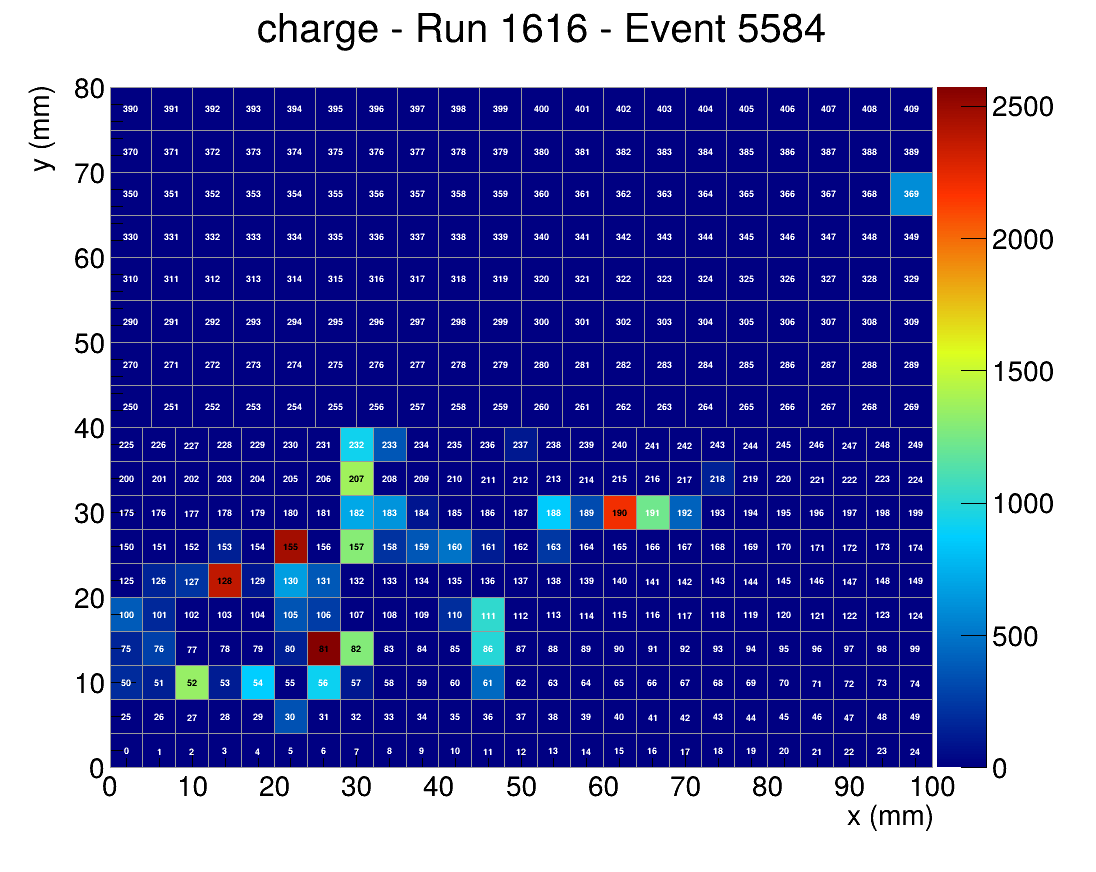
\includegraphics[width=.85\linewidth]{figures/event_charge.png}
\caption{Run 1616, event 5584: numbered physical charge display.}
\end{figure}
\begin{figure}[p]
\centering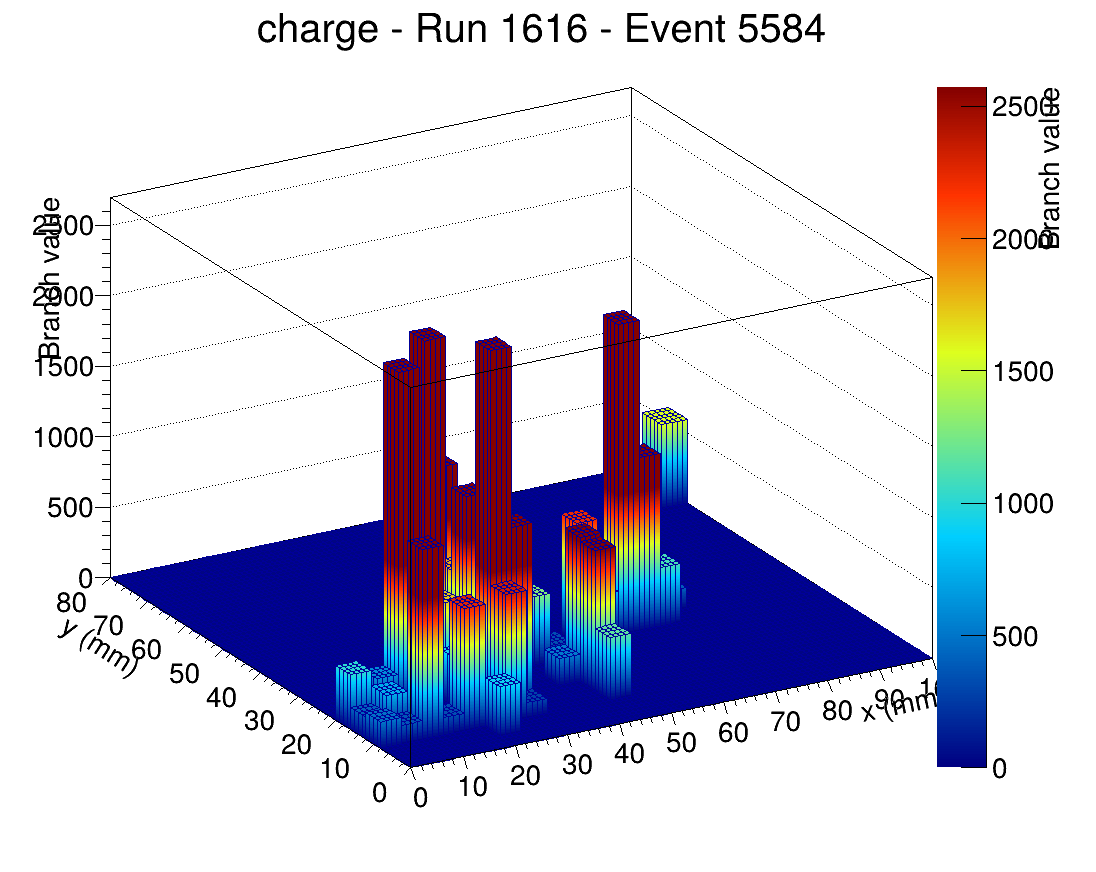
\includegraphics[width=.85\linewidth]{figures/event_charge_3d.png}
\caption{The same event in 3D. Heights are displayed values; no track reconstruction is performed.}
\end{figure}

\section{Independent voltage study}
This workflow uses detector cleaning from \texttt{run\_cuts.ini} and then adds
\texttt{voltage\_study\_cuts.ini}. Only this study opens that second file. Its
channel-range restriction is independent of normal raw/cleaned/event inspection.
\begin{lstlisting}
root -l -b -q 'analysis_root/TPC.C("voltage")'
python analysis/tpc.py voltage
python analysis/tpc.py voltage --study-cuts-db config/voltage_study_cuts.ini
\end{lstlisting}
The run/voltage table is \texttt{data/datafiles-voltage.txt} for Python and the
ROOT auxiliary copy for ROOT. Conflicting voltage assignments are excluded until
corrected (Python also has \texttt{-{}-voltage-override RUN=VOLTS}). Repeated voltages
select the eligible file with most distinct events before cuts; ties use clean event
count and then the lower run ID. Excluded scan runs are configured in settings.

Count overlays preserve accepted pulse totals. Unit-area overlays compare shapes
by dividing by accepted-hit count. Neither is a live-time normalization. Histograms
count all accepted pulses. The occupancy/audit plots explain detector-wide and
module-flooding vetoes. Output goes to \texttt{results/ENGINE/voltage/}, including
histograms, run summaries and rejected-event evidence. Both parsed cut files are
snapshotted separately. Extend the voltage histogram's \texttt{time\_max} setting
if you expand the accepted Time range.

\begin{figure}[p]
\centering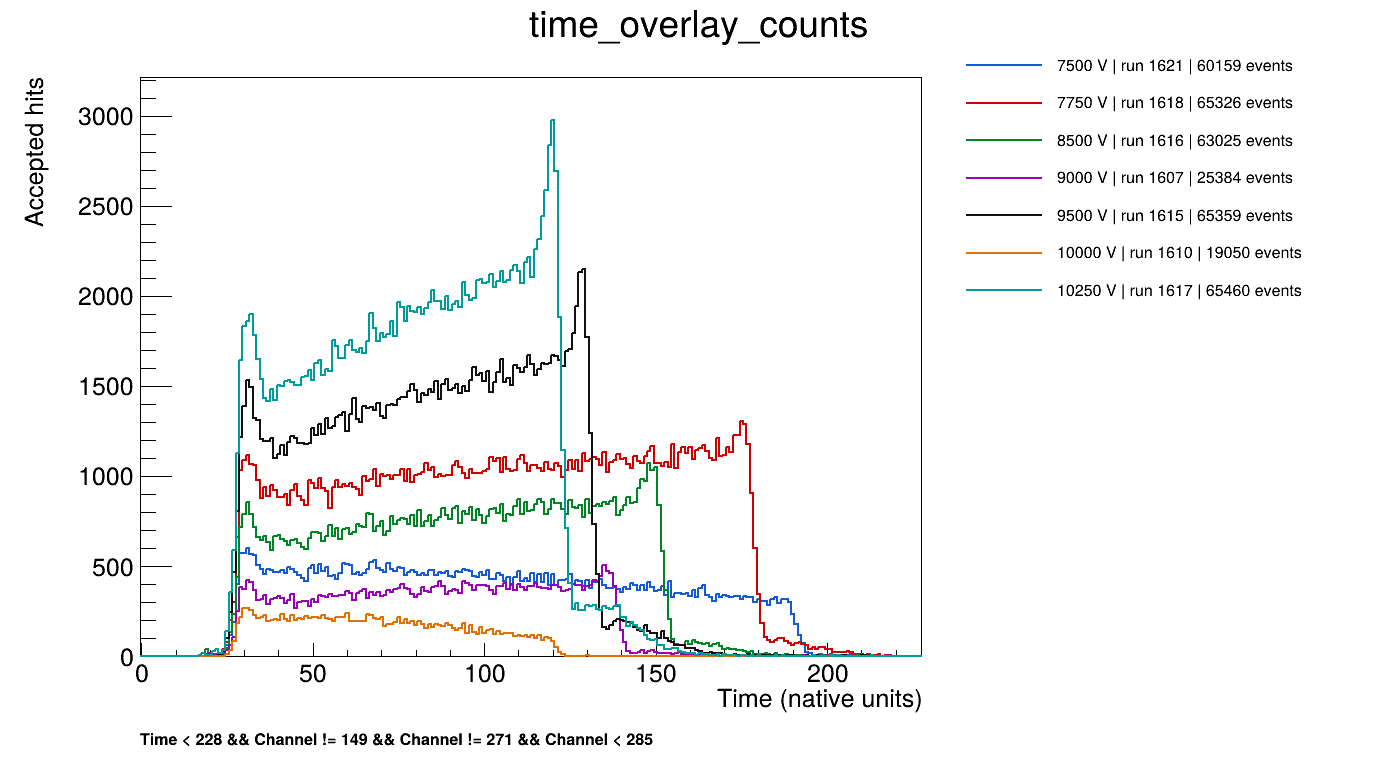
\includegraphics[width=\linewidth]{figures/voltage_overlay.png}
\caption{Reference independent voltage-study example: time histograms from runs at different
voltages, with detector and study cuts and automatic event vetoes. One eligible run
per voltage is selected. This multi-run illustration requires additional data beyond
the bundled single-run example.}
\end{figure}

\section{Files, reproducibility and custom locations}
Raw 1D files: \texttt{raw\_histograms.root}, overview/individual PNG/PDFs,
per-quantity bin CSVs and summary (Python JSON, ROOT CSV).
Raw 2D files: \texttt{2d/raw\_2d\_histograms.root}, overview/individual PNG/PDFs,
sparse bin CSVs and summary. Both carry native editable histograms and TCanvas
objects. Reopen a ROOT file and use \texttt{new TBrowser;} to inspect its keys.
Clean exports include \texttt{cuts\_used.ini}; the voltage study additionally saves
\texttt{voltage\_study\_cuts\_used.ini}. Snapshots describe the version actually used,
so older exports can legitimately carry older configuration text.
\begin{lstlisting}
root -l results/root/raw/run1616/raw_histograms.root
// At the ROOT prompt:
new TBrowser;

python analysis/tpc.py raw 1616 --input-dir /path/to/rootfiles --output-dir /path/to/output
python analysis/tpc.py raw 1616 --apply-cuts --cuts-db /path/to/cuts.ini --veto-file /path/to/veto.csv
\end{lstlisting}
An alternate detector DB completely replaces the default, including global cuts.
The ROOT interface has the following optional positional parameters; empty strings
retain defaults:
\begin{lstlisting}
TPC(command, run, event, inputDirectory, outputDirectory,
    vetoCSV, cutsDB, studyCutsDB);
// Example export with alternate input and detector DB:
TPC("save",1616,5584,"/path/to/data","/path/to/output","","/path/to/cuts.ini");
\end{lstlisting}

\section{Custom ROOT palette}
The \texttt{set\_color\_env()} function is defined near the top of \texttt{TPC.C} and is now
called in \texttt{TPC(...)} immediately after \texttt{SetOptStat(0)}, before drawing:
\begin{lstlisting}
gStyle->SetOptStat(0);
set_color_env();
\end{lstlisting}
Edit its stops and RGB arrays to change the continuous palette; NCont controls the
number of colour levels. A later \texttt{SetPalette(kViridis)} would override it,
Explicit curve/line colours
(e.g. voltage overlays) are set separately. Python Matplotlib uses its own cmap
settings; the C++ function controls the ROOT workflow.
\lstinputlisting[basicstyle=\ttfamily\scriptsize]{generated/palette.C}

\section{Where to modify the implementation}
\begin{longtable}{p{.33\linewidth}p{.6\linewidth}}
\texttt{analysis/tpc.py} & Commands/menu, common inspection context, 1D/2D drawing, event display styles and exports.\\
\texttt{analysis/detector.py} & ROOT input, wiring, rejection parser/masks, event noise, CSV/axis definitions.\\
\texttt{analysis/voltage.py} & Independent voltage study, normalization, run choice and audits.\\
\texttt{analysis\_root/TPC.C} & Public dispatcher (Section 10), drawing/export functions, palette; Sections 8B/8C implement 1D/2D inspection.\\
\texttt{analysis\_root/TPCDetector.h} & Native input, mapping, cuts, geometry and noise classification.\\
\end{longtable}
For later reconstruction preserve all passing pulses using the hit mask (Python)
or raw Hit records and PassHit (ROOT). Mapping supplies pad centres/footprints.
DisplayHits/first-pulse reduction is a visualization choice. Drift calibration,
reference time, spatial fitting and track output require separate future work.

\clearpage\appendix
\section{Current configuration snapshots}
These are the exact files copied at manual build time. Edit the originals in
\texttt{config/}, not these generated copies.
\subsection{Detector cuts}
\lstinputlisting[basicstyle=\ttfamily\scriptsize]{generated/run_cuts.ini}
\subsection{Independent study cuts}
\lstinputlisting[basicstyle=\ttfamily\scriptsize]{generated/voltage_study_cuts.ini}
\subsection{1D binning}
\lstinputlisting[basicstyle=\ttfamily\scriptsize]{generated/raw_binning.csv}
\subsection{2D pair definitions}
\lstinputlisting[basicstyle=\ttfamily\scriptsize]{generated/raw_2d_plots.csv}
\subsection{Python automatic-noise and histogram settings}
\lstinputlisting[basicstyle=\ttfamily\scriptsize]{generated/analysis_settings.csv}
\subsection{ROOT automatic-noise and histogram settings}
\lstinputlisting[basicstyle=\ttfamily\scriptsize]{generated/analysis_root_settings.csv}
\section{Current Python command help}
\subsection{Inspection}
\lstinputlisting[basicstyle=\ttfamily\scriptsize]{generated/raw_help.txt}
\subsection{Event display}
\lstinputlisting[basicstyle=\ttfamily\scriptsize]{generated/event_help.txt}
\subsection{Independent voltage study}
\lstinputlisting[basicstyle=\ttfamily\scriptsize]{generated/voltage_help.txt}
\end{document}
